\newpage

\section{Feature description}

\subsection{Motivation}
It has recently been demonstrated that local feature descriptors
based on convolutional neural networks (CNN) can significantly
improve the matching performance.  Previous work on learning such
descriptors has focused on exploiting pairs of positive and negative
patches to learn discriminative CNN representations. In this work,
we propose to utilize triplets of training samples, together with
in-triplet mining of hard negatives. We show that our method
achieves state of the art results, without the computational
overhead typically associated with mining of negatives and with
lower complexity of the network architecture.  We compare our
approach to recently introduced convolutional local feature
descriptors, and demonstrate the advantages of the proposed methods
in terms of performance and speed.  We also examine different loss
functions associated with triplets.

%%%%%%%%% INTRO
\subsection{Introduction}

Finding correspondences between images via local descriptors is one of
the most extensively studied problems in computer vision due to the
wide range of applications. The field has witnessed several
breakthroughs in this area such as
SIFT~\cite{Lowe:2004:DIF:993451.996342}, invariant region
detectors~\cite{mikolajczykIJCV2004}, fast binary
descriptors~\cite{Calonder:2010:BBR:1888089.1888148}, optimised
descriptor parameters \cite{WHB09,simonyan2014learning} which have
made a significant and wide impact in various computer vision tasks.
Recently end-to-end learnt
descriptors~\cite{FDB14,simo2015deepdesc,ZagoruykoCVPR2015,Han_2015_CVPR}
based on CNN architectures and training on a large dataset of positive
and negative sample pairs, were demonstrated to significantly
outperform state of the art features. This was a natural adoption of
CNN to local descriptors as deep learning had already been shown to
significantly improve in many computer vision areas
\cite{lecun2015deep}.

Recent work on deep learning for learning feature embeddings examines
the use of triplets of samples instead of solely focusing on pairs
\cite{DBLP:journals/corr/WangSLRWPCW14,DBLP:journals/corr/HofferA14,wohlhart15}.
Different loss functions are proposed in these works, but a systematic
study of their characteristics is yet to be done. In addition, these
works are focused on more general embeddings (e.g. product similarity,
3D description of objects, MNIST classification). In this work, we
investigate the use of triplets in learning local feature descriptors
with convolutional neural networks. Other contributions include: 1) we
examine different different loss functions for triplet based-learning,
2) we investigate the performance of these methods in terms of patch
matching, and patch pairs classification in widely used benchmarks, 3)
we show that in-triplet hard negative mining can lead to improved
results, 4) we demonstrate that excellent descriptor performance can
be obtained with a shallow network thus avoiding computationally
complex architectures and expensive mini-batch hard negative mining.

\subsection{Related work}
The design and implementation of local descriptors has undergone a
remarkable evolution over the past two decades ranging from
differential or moment invariants, correlations, PCA projected patches, histograms of
gradients or other measurements, etc. An
overview of  pre-2005 descriptors with SIFT
\cite{Lowe:2004:DIF:993451.996342} identified as the top performer can
be found in \cite{schmid2003performance}. 
Its benchmark data accelerated the progress in this field and there
have been a number of notable contributions, including recent DSP-SIFT
\cite{DBLP:journals/corr/DongS14}, falling into the same category of
descriptors as SIFT but the improvements were not sufficient to
supersede SIFT in general. The research focus shifted to
improve the speed and memory footprint e.g. as in BRIEF
\cite{Calonder:2010:BBR:1888089.1888148} and the follow up efforts.
Introduction of datasets with correspondence ground truth \cite{WHB09}
stimulated development of learning based descriptors which try to
optimise descriptor parameters and learn projections or distance
metrics \cite{BHW10,simonyan2014learning} for better matching. 

End-to-end learning of patch descriptors using CNN has been attempted
in several works
\cite{FDB14,ZagoruykoCVPR2015,simo2015deepdesc,Han_2015_CVPR} and
consistent improvements were reported over the state of the art
descriptors.  Interest in the field started from results shown in
\cite{FDB14} that the features from the last layer of a convolutional
deep network trained on ImageNet \cite{ILSVRC15} can outperform
SIFT. This was a significant result, since the convolutional features
from ImageNet were not specifically learnt for such local
representations.

Learning a CNN from local patches extracted from
local features only, based on a siamese architecture with hinge
contrastive loss \cite{1640964} was demonstrated in
\cite{ZagoruykoCVPR2015,simo2015deepdesc,Han_2015_CVPR} to significantly
 improve the matching performance. This approach was originally proposed in \cite{Jahrer}, however due to the limited evaluation this work was
not immediately followed.

Note that in ~\cite{ZagoruykoCVPR2015,Han_2015_CVPR} both feature
layers and metric layers are learnt in the same network. Thus, the
final contrastive loss is optimised in terms of the abstract metric
learned in the last layer of the network. On the contrary,
~\cite{simo2015deepdesc} directly uses the features extracted after
the convolutional layers of the CNN, without training a specialised
distance layer. This allows the extracted descriptors to be used in
traditional pipelines. However, the experiments from
\cite{ZagoruykoCVPR2015} show that metric learning performs better
than generic $L2$ matching. In our experiments, we also use features
from CNNs without any metric learning layer.

Another important observation from \cite{ZagoruykoCVPR2015} is that
multiscale architectures perform better than the single scale ones. However,
this is not unique to the CNNs, since previous works have
shown that aggregating descriptors from multiple scales, improves the
results.  We focus on single scale architectures,
since these are the building blocks for multiscale descriptors, and
improving them, will improve the final multiscale results as argued
by the DSP theory from \cite{DBLP:journals/corr/DongS14}.

\subsection{Learning patch descriptors}

In this section, we first discuss the two most commonly used loss functions when learning with triplets, and we then investigate their characteristics.  A patch descriptor is considered as  a non-linear encoding resulting from a final layer of a convolutional neural network. Let
$\boldsymbol x \in \mathbb{R}^{n \times n}$ represent the patch given
as input to the network, and $f(\boldsymbol x) \in \mathbb{R}^{D}$
represent the $D$ features given as output from the network.
For all of the methods below, the goal is to learn the embedding
$f(\boldsymbol x)$ s.t. $||f(\boldsymbol x_1) - f(\boldsymbol x_2)
||_2$ is low if $\boldsymbol x_1$ and $\boldsymbol x_2$ are extracted from the same physical point location i.e. positive match, and high otherwise.

\subsubsection{Learning with pairs}
Learning with pairs involves training from samples of the form
$\{\boldsymbol x_1,\boldsymbol x_2,\ell\}$, with  $\ell$ being 
 a label for the patch pair, which is $-1$
for negative pairs, and $1$ for positive pairs. The contrastive loss is defined as 
\begin{equation}
  \label{eq:contrastive-loss}
  l(\boldsymbol x_1,\boldsymbol x_2;\ell) =
\left\{
	\begin{array}{ll}
		||f(\boldsymbol x_1)-f(\boldsymbol x_2)||_2  & \mbox{if } \ell=1 \\
		max(0,\mu-||f(\boldsymbol x_1)-f(\boldsymbol x_2)||_2)  & \mbox{if } \ell=-1
	\end{array}
\right.
\end{equation}
where $\mu$ is an arbitrarily set margin. Note that the
weights of the CNN in $f(\cdot)$ need to be regularised, otherwise the margin would
have no effect. Intuitively the hinge embedding loss penalizes positive pairs
that have large distance and negative
pairs that have small distance (less than $\mu$).

Note that learning local feature descriptors is a more specific
problem than general image classification such as in ImageNet, since
the transformations a local patch can undergo are limited compared to
different objects of the same visual category. In addition, patches in
pairs representing negative examples are usually very different, thus
make it easy for the learning process to optimize the distances. This
issue is identified in \cite{simo2015deepdesc}, where the majority of
the negative patch pairs ($\ell=-1$) do not contribute to the update
of the gradients in the optimization process as their distance is
already larger than $\mu$ parameter in
Eq. \eqref{eq:contrastive-loss}. To address this issue hard negative
mining was proposed \cite{simo2015deepdesc} to include more negative
pairs in the training. The hard negative training pairs were
identified by their distance and a subset of these examples were
re-fed to the network for gradient update in each iteration. Note that
while this process leads to more discriminative convolutional
features, it also comes at a very high computational cost, since in
each epoch, a subset of the training data need to be backpropagated
again through the network. Specifically, the best performing
architecture from \cite{simo2015deepdesc}, required $67\%$ of the
computational cost to be spent for mining hard negatives.


\subsubsection{Learning with triplets}
Recent work in~\cite{DBLP:journals/corr/HofferA14}
shows that learning representations with triplets of examples, gives much better results than
learning with pairs using the same network. Inspired by this, we  focus on learning feature descriptors based on triplets of  patches.

Learning with triplets involves training from samples of the form
$\{\boldsymbol a,\boldsymbol p,\boldsymbol n \}$, where $a$ is the
\textit{anchor}, $p$ \textit{positive}, which is a different sample of the
same class as $a$, and $n$ \textit{negative} is a sample
belonging to a different class. In our case, $a$ and $p$ are different
viewpoints of the same physical point, and $n$ comes from
a different keypoint. Furthermore, optimising the parameters of the
network  brings $a$ and $p$ close in the feature space, and pushes $a$ and $n$ far apart.  For
brevity, we shall write that
$\delta_{+} = ||f(\boldsymbol a)-f(\boldsymbol p)||_2$ and
$\delta_{-} = ||f(\boldsymbol a)-f(\boldsymbol n)||_2$. We can
categorise the loss functions that have been proposed in the
literature for learning convolutional embeddings with triplets into
two groups, the {\em ranking-based losses} and the {\em ratio-based
  losses}
\cite{wohlhart15,DBLP:journals/corr/HofferA14,DBLP:journals/corr/WangSLRWPCW14}. Below
we give a brief review of both categories, and  discuss their
differences.

\textbf{Margin ranking loss.}
This ranking loss that was first proposed for learning embeddings using
convolutional neural networks in
\cite{DBLP:journals/corr/WangSLRWPCW14} is defined as
 
\begin{equation}
  \label{eq:triplet-margin}
  \lambda(\delta_+,\delta_-) = max(0, \mu
		+\delta_+-\delta_-) 
\end{equation}
where $\mu$ is a margin parameter.  The margin ranking loss is a
convex approximation to the $0-1$ ranking error loss, which measures
the violation of the ranking order of the embedded features inside in
the triplet. The correct order should be
$\delta_{-} > \delta_{+} + \mu$. If that is not the case, then the
network adjusts its weights to achieve this result. As it can be seen
the formulation also involves a margin, similarly to
Eq.\eqref{eq:contrastive-loss}. Note that if this marginal distance
difference is respected, the loss is 0, and thus the weights are not
updated. Fig.~\ref{fig:losses} (b) illustrates the loss surface of
$\lambda(\delta_+,\delta_-)$. The loss remains 0 until the margin is
violated, and after that, there is a linear increase. Also note that
the loss in not upper bounded, only lower bounded to 0.

\textbf{Ratio loss.} In contrast to the ranking loss that forces the embeddings to be learned such that they satisfy ranking of the form
$\delta_{-}>\delta_{+}+\mu$, a ratio loss is investigated in
\cite{DBLP:journals/corr/HofferA14} which optimises the ratio
distances within triplets. This loss learns embeddings such that
$\frac{\delta_{-}}{\delta_{+}}\rightarrow \infty$.

\begin{equation}
  \label{eq:triplet-ratio}
  \hat{\lambda}(\delta_+,\delta_-) = (\frac{e^{\delta_+}}{e^{\delta_+}+e^{\delta_-}})^2+(1-\frac{e^{\delta_-}}{e^{\delta_+}+e^{\delta_-}})^{2}
\end{equation}
As one can examine from Eq.~\ref{eq:triplet-ratio}, the goal of this
loss function is to force
$(\frac{e^{\delta_+}}{e^{\delta_+}+e^{\delta_-}})^2$ to $0$, and
$(\frac{e^{\delta_-}}{e^{\delta_+}+e^{\delta_-}})^2$ to $1$. Note that
both are achieved by the first term of the equation, but we
report here the original formulation from
\cite{DBLP:journals/corr/HofferA14}.  There is no margin associated
with this loss, and by definition we have
$0 \leq \hat{\lambda} \leq 1$ for all values of
$\delta_{-},\delta_{+}$.  Note that unlike the margin-ranking loss,
where $\lambda=0$ is possible, every training sample in this case is
associated with some non-negative loss value.  Fig.~\ref{fig:losses}
(d) shows the loss surface of $\hat{\lambda}(\delta_+,\delta_-)$,
which compared to the ranking based loss has a clear slope between the
two loss levels, and the loss reaches a plateau quickly when
$\delta_{-} > \delta_{+}$. Also note that this loss is upper bounded
to $1$.

% \begin{figure}
% \centering    
% \subfigure[]{ \resizebox{0.12\textwidth}{!}{
%             \begin{tikzpicture}
%               \draw (2,2) circle (1.5cm);
%               \draw[dashdotted, very thin] (2,2) -- (1.55,3.3)
%               node[midway,right] {\Large$\delta_{-}$};
%               \draw[-, very thin,orange] (2.15,2) -- (3.5,2)node[midway, below,black]{\Large $ \mu$};              \draw[-, very thin] (2,2) -- (2.2,0.8) node[midway,left] {\Large$\delta_{+}$};
%               \draw [draw=black, fill=gray] (2,2) circle (0.4cm) ;
%               \node[draw=none,text=white] at (2,2) {\Large $a$};
%               \draw [draw=black, fill=red] (1.4,3.5) circle (0.4cm) ;
%               \node[draw=none,text=black] at (1.4,3.5) {\Large $n$};
%               \draw [draw=black, fill=blue] (2.2,0.8) circle (0.4cm);
%               \node[draw=none,text=white] at (2.2,0.8) {\Large $p$};
%             \end{tikzpicture}}}
% \subfigure[]{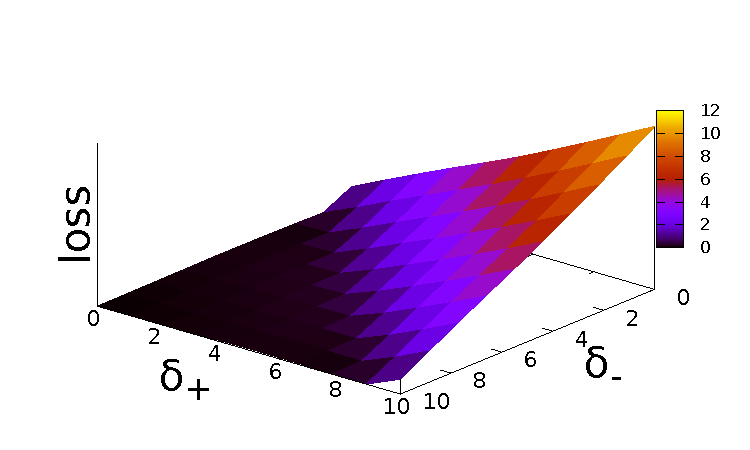
\includegraphics[width=0.27\textwidth]{main/chapter02/images/margin.pdf}}
% \quad
% \subfigure[]{ \resizebox{0.12\textwidth}{!}{
%     \begin{tikzpicture}
%       \draw[-, very thin] (1,1.5) -- (3,3);
%       \draw[dashdotted, very thin] (1,1.5) -- (1.9,3);
%       \draw [draw=black, fill=gray] (1,1.5) circle (0.4cm) ;
%       \node[draw=none,text=white] at (1,1.5) {\Large $a$};
%       \draw [draw=black, fill=red] (3,3) circle (0.4cm) ;
%       \node[draw=none] at (3,3) {\Large $p$};
%       \draw [draw=black, fill=blue] (1.9,3) circle (0.4cm) ;
%       \node[draw=none,text=white] at (1.9,3) {\Large $n$};
%       \node[draw=none] at (2.3,2) {\large $\delta_{+}$};
%       \node[draw=none] at (1,2.4) {\large $\delta_{-}$};
%     \end{tikzpicture}}}
% \subfigure[]{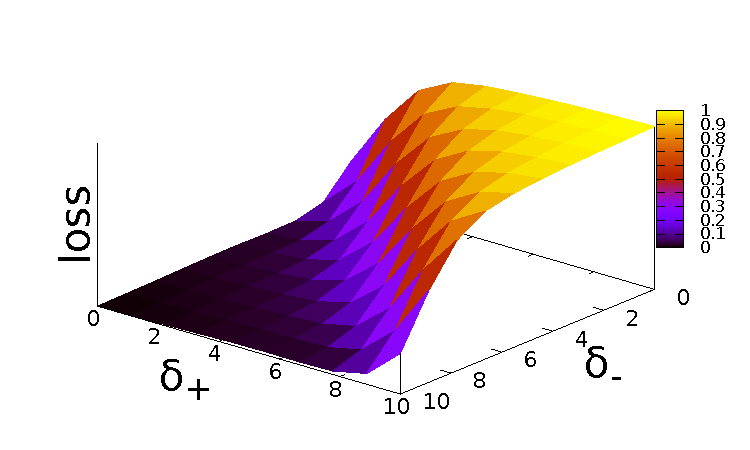
\includegraphics[width=0.27\textwidth]{main/chapter02/images/ratio.pdf}}
% \caption{(a) Margin ranking loss. It seeks to push $n$ outside
%   the circle defined by the margin $\mu$, and pull $p$ inside. (b)
%   Margin ranking loss values in function of $\delta_{-},\delta_{+}$
%   (c) Ratio loss. It seeks to force
%   $\delta_{+}$ to be much smaller than $\delta_{-}$. (d)
%   Ratio loss values in function of $\delta_{-},\delta_{+}$}
% \label{fig:losses}
% \vspace{-0.2cm}
% \end{figure}

\begin{figure}[t]
    \centering
    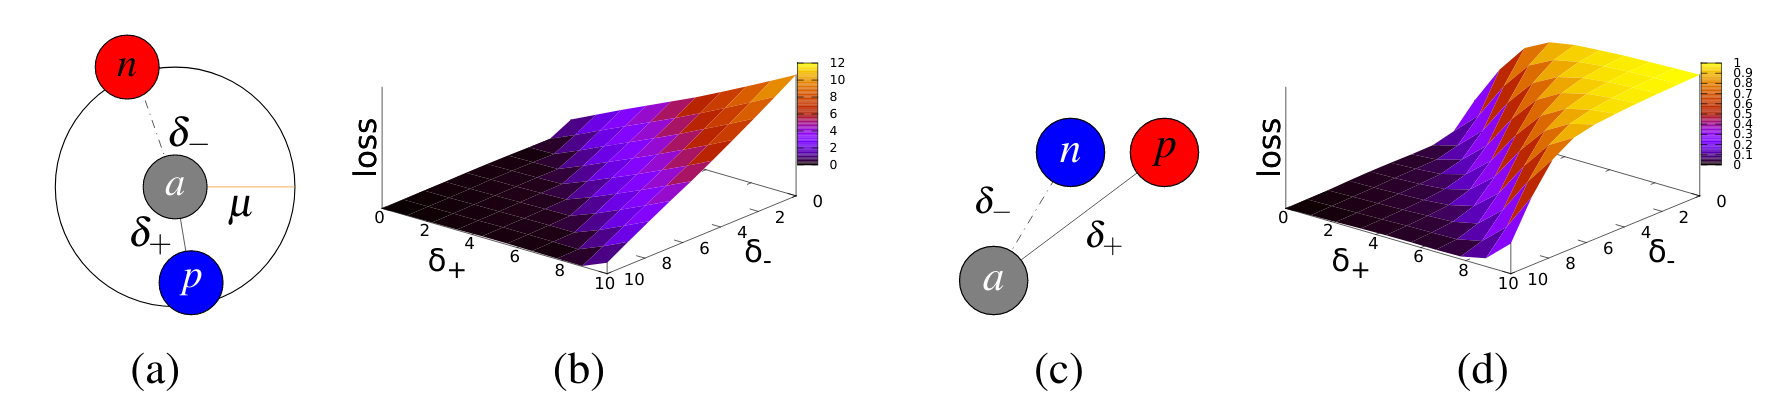
\includegraphics[scale=0.19]{main/chapter02/images/tfeat_losses.png}
    \caption{(a) Margin ranking loss. It seeks to push $n$ outside
  the circle defined by the margin $\mu$, and pull $p$ inside. (b)
  Margin ranking loss values in function of $\delta_{-},\delta_{+}$
  (c) Ratio loss. It seeks to force
  $\delta_{+}$ to be much smaller than $\delta_{-}$. (d)
  Ratio loss values in function of $\delta_{-},\delta_{+}$}
\label{fig:losses}
\end{figure}  


\subsubsection{In-triplet hard negative mining with anchor swap}

All previous works that exploit the idea of triplet based learning use only two of
the possible three distances within each triplet w.r.t. one
sample  used as an \textit{anchor}, thus ignoring the
third distance 
$\delta_{-}^{'} = ||f(\boldsymbol p)-f(\boldsymbol n)||_2.$ Note that
since the feature embedding network already computes the
representations for
$f(\boldsymbol a), f(\boldsymbol p), f(\boldsymbol n) $, there is no
need for extra convolutional overhead to compute
$\delta_{-}^{'}$ except
evaluating the $L_2$ distance.

We define the \textit{in-triplet hard negative} as
$\delta_{*} = min(\delta_{-},\delta_{-}^{'})$. If
$\delta_{*} = \delta_{-}^{'}$, we swap $\{a,p\}$, and thus $p$ becomes
the \textit{anchor}, and $a$ becomes the \textit{positive}
sample. This ensures that the hardest negative inside the triplet 
is used for backpropagation. Subsequently, the margin ranking loss
becomes $\lambda(\delta_+,\delta_*) = max(0, \mu
+\delta_+-\delta_*)$. A similar expression can be devised for the
ratio loss.  This simple technique can lead to improved
results without  computational overhead, as we experimentally show in section~\ref{sec:patch_classification}. 

\subsubsection{Implementation details}

To demonstrate the impact that triplet based training has on the performance of CNN descriptors we use a simple network architecture :
\{Conv(7,7)-Tanh-Pool(2,2)-Conv(6,6)-Tanh-FC(128)\} implemented in
\texttt{Torch} \cite{collobert:2011c} with the following simplified training process. 
CNN is trained from $5M$
triplets sampled on-the-fly using patches from
\cite{BHW10}. We do not use data
augmentation unlike in typical CNNs for general classification or convolutional feature descriptors from
\cite{ZagoruykoCVPR2015}\cite{Han_2015_CVPR}.  When forming a triplet for training we choose randomly a positive
pair of patches that originate from the same  physical point and  a
randomly sampled patch from another keypoint. This is in contrast to
other works where carefully designed schemes of choosing the training
data are used in order to enhance the
performance~\cite{DBLP:journals/corr/WangSLRWPCW14,Han_2015_CVPR}.
For the optimization the Stochastic Gradient Descend
\cite{bottou-tricks-2012} is used, and the training is done in batches
of $128$ items, with a learning rate of $0.1$ which is temporally
annealed, momentum of $0.9$ and weight decay of $10^{-6}$. We also
reduce the learning rate every epoch. The convolution methods are from
the NVIDIA cuDNN library \cite{DBLP:journals/corr/ChetlurWVCTCS14}.
The training of a single epoch with $5M$ training triplets takes
approximately $10$ minutes in an NVIDIA Titan X GPU.

It is worth noting that the CNN used in our experiments consists of
only two convolutional layers, while all of the other state-of-the art
deep feature descriptors consist of four or more layers
\cite{ZagoruykoCVPR2015,simo2015deepdesc,Han_2015_CVPR}.  Our
motivation for such shallow network is to develop a descriptor for
practical applications including those requiring real time
processing. This is a challenging goal given that all previously
introduced descriptors are computationally very intensive, thus
impractical for most applications.  This design is also inspired by
the approach introduced in \cite{simonyan2014learning}, where pooling
of the responses of Gaussian filters and a simple linear projection
produced very good results. Thus, we build a simple hierarchical
network that is based on $100$ convolutional filters, followed by a
linear transformation that projects the responses of the filters to
the desired output dimensionality.  Several other implementation
variants are possible such as different non-linearity layers
(e.g. ReLU as in \cite{Han_2015_CVPR,ZagoruykoCVPR2015}), extra
normalization layers, or multiscale architectures but these are likely
to further improve the results and are beyond the scope of this work.

\subsection{Experimental evaluation}

In this section we evaluate the proposed local feature descriptor
within the two most popular benchmarks in the field of local
descriptor matching and we test on different datasets to show
that it can generalise well. We compare our method to SIFT
\cite{Lowe:2004:DIF:993451.996342}, Convex optimization
\cite{simonyan2014learning} and the recently introduced convolutional
feature descriptors MatchNet \cite{Han_2015_CVPR}, DeepCompare
\cite{ZagoruykoCVPR2015} and DeepDesc \cite{simo2015deepdesc}, which
are currently the state of the art in terms of matching accuracy.  The
original code  was used in all the experiments. More details can be found in the supplementary
materials. We name our four variants \texttt{TFeat-ranking} for the
networks learnt with the ranking loss, \texttt{TFeat-ranking*} for
the networks learnt with the ranking loss with anchor swap,
\texttt{TFeat-ratio} for the ratio loss, and \texttt{TFeat-ratio*} for the
ratio loss with anchor swap.

Note that for a fair comparison, we do not use the multi-scale {\em
  2ch architectures} from \cite{ZagoruykoCVPR2015}. Multi-scale
approaches use multiple patches from each example, with extra inputs
in form of cropped sub-patches around the center of each patch. This
introduces information from different samples in the scale-space and
it has been shown to lead to significant improvements in terms of
matching accuracy \cite{DBLP:journals/corr/DongS14}. Such approach can
be used for various descriptors (e.g. MatchNet-2ch, TFeat-2ch,
DeepDesc-2ch). The evaluation is done with two different evaluation
metrics frequently found in the literature, patch pair classification
success in terms of ROC curves \cite{WHB09}, and mean average
precision in terms of correct matching of feature points between pairs
of images \cite{schmid2003performance}. Note that these two metrics
are of very different nature, the former measures how succesfull a
classification of positive and negative patch pairs is, and the latter
is evaluating the performance of a descriptor in nearest neighbour
matching scenario where the task is to find correspondences in two
large sets of descriptors.

\subsubsection{Patch pair classification}
\label{sec:patch_classification}
The patch pair classification benchmark measures the ability of
a descriptor to discriminate positive patch pairs from negative ones in
the Photo Tour dataset \cite{BHW10}. This dataset consists of three
subsets {\em Liberty},{\em Yosemite} \& {\em Notredame}, with each
containing more than 500k patch pairs extracted around  keypoints.  We follow the protocol proposed in \cite{BHW10} where
the ROC curve is generated by thesholding the distance scores between
patch pairs. The number reported here is the false positive rate at
95\% true positive rate (FPR95), as used in many influencial works in
the field. For the evaluation we use the $100K$ patch pairs proposed as defined in the benchmark.  Note that 
DeepDesc~\cite{simo2015deepdesc}, does not report performance with training
based on a single dataset, therefore for each test set, the training is
performed on the other two datasets.

The results for each of the combinations of training and testing using
the three subsets of the Photo Tour dataset are shown in
Table~\ref{tab:benchmark_brown} including the average across all possible
combinations. Our networks outperform all
the previously introduced single-scale convolutional feature
descriptors, and in some cases with large margins except from one
training-test combination where the 4096-dimensional version of
MatchNet outperforms our TFeat variants. However, even in this
case, the version of MatchNet with comparable dimensionality to our
descriptors is outperformed by three of our variants. Also note that
MatchNet is specifically designed for patch pair classification,
since it also includes a similarity metric layer  trained on top of the feature layer.

%A possible explanation for this
%phenomenon is the fact that the Notredame patches are very high in
%detail, something that might discourage the ratio criterion. 

\begin{table*}[ht]
\begin{tabular}{lcccccccc}
\toprule 
    Training& & Not & Lib & Not  & Yos & Yos
  & Lib  & \\
    % \midrule
    Testing&  &
                \multicolumn{2}{c}{Yos} & \multicolumn{2}{c}{Lib} & \multicolumn{2}{c}{Not} \\
    \midrule
    Descriptor & \# & & & & & & &mean  \\
    \midrule
    {\small SIFT} \cite{Lowe:2004:DIF:993451.996342} & 128 & \multicolumn{2}{c}{27.29} & \multicolumn{2}{c}{29.84}
                                    & \multicolumn{2}{c}{22.53} &
                                                                  26.55
  \\
   {\small ImageNet$_{4conv}$} \cite{FDB14} & 128 & \multicolumn{2}{c}{30.22} & \multicolumn{2}{c}{14.26}
                                    & \multicolumn{2}{c}{9.64} & 18.04
                                                                   \\
    {\small ConvexOpt} \cite{simonyan2014learning} & 80 & 10.08 & 11.63
                                    & 11.42 & 14.58 & 7.22 & 6.17 &
                                                                    10.28
  \\
     {\small DeepCompare} {\scriptsize siam} \cite{ZagoruykoCVPR2015}& 256 &
                                 15.89                                     
                          & 19.91 & 13.24 & 17.25 & 8.38 & 6.01 & 13.45 
  \\
      {\small Deepcompare} {\scriptsize {\it siam2stream}}& 512 & 13.02
                          & 13.24 & 8.79 & 12.84 & 5.58 & 4.54 & 9.67 \\
   {\small DeepDesc} \cite{simo2015deepdesc} & 128 & \multicolumn{2}{c}{16.19} & \multicolumn{2}{c}{8.82}
                                    & \multicolumn{2}{c}{4.54} & 9.85
                                                                   \\
    {\small MatchNet} \cite{Han_2015_CVPR} & 512 & 11 & 13.58
                                    & 8.84 & 13.02 & 7.7 & 4.75 & 9.82\\
    {\small MatchNet} \cite{Han_2015_CVPR} & 4096 & 8.39 & 10.88
                                    &
                                      \bf 6.90 & 10.77 & 5.76 & 3.87 & 7.75\\
 {\em TFeat-ratio} &  128 & \bf 8.32 & \bf 10.25 &  8.93 & \bf 10.13  & \bf 4.12  &  \bf 3.79 & \bf 7.59  \\
 {\em TFeat-ratio*} &  128 & \bf 7.24 & \bf 8.53 &  8.07 & \bf 9.53  & \bf 4.23 & \bf 3.47 & \bf 6.84  \\
 {\em TFeat-margin} &  128 & \bf 7.95 & \bf 8.10 &  7.64 &  \bf 9.88 & \bf 3.83  & \bf 3.39  & \bf 6.79 \\ 
 {\em TFeat-margin*} &  128 & \bf 7.08 & \bf 7.82 & 7.22 &  \bf 9.79  &  \bf 3.85  &  \bf 3.12 & \bf 6.47 \\ 
  \bottomrule
\end{tabular}
  \caption {Results form the Photo-Tour dataset \cite{BHW10}. Numbers
    are reported in terms of {\em FPR95} following state of the art 
    in this field (see text for more details). {\em Italics} indicate
    the descriptors introduced here, and {\bf bold} numbers indicate
    the top performing descriptor. Yos:Yosemite, Lib:Liberty,
    Not:Notredame.}
\label{tab:benchmark_brown} 
\end{table*}

\subsubsection{Nearest neighbour patch matching}

To measure the nearest neighbour matching performance, we establish
correspondence ground truth using the homographies and the overlap
error from \cite{schmid2003performance}.  We consider two feature
points between the two images in correspondence if the overlap error
between the detected regions is less than 50\%.  Note that a region
from one image can be in correspondence with several regions from the
other image.  Each image has an associated set of approximately 1K
patches.  The results are presented with precision-recall curves as it
was originally proposed in \cite{schmid2003performance}.  More
specifically, for each patch from the left image we find its nearest
neighbour in the right image.  Based on the ground truth overlap we
identify the false positives and true positives, and generate
precision-recall curves. The area under the precision-recall curve is
the reported mean-average precision
\cite{WHB09,ZagoruykoCVPR2015,DBLP:journals/corr/DongS14}.  For this
experiment, we use the \texttt{vl\_benchmarks}~\cite{vedaldi08vlfeat} library
(\texttt{vl\_covdet} function), with some minor modifications to limit
the descriptors extracted from an image to 1K, which is important to
avoid bias by different numbers of features in different images. For
all the experiments below, the descriptors are trained on Liberty-DoG
patches \cite{BHW10}.

For the nearest neighbor matching test two datasets are mainly used in
the literature, {\em Oxford matching dataset}
\cite{schmid2003performance}, which is of small size, but include
images acquired by a camera, and the {\em generated matching dataset}
\cite{FDB14} which is much larger in volume but created
synthetically. In the following sections, we discuss our results in
those two datasets.

\textbf{Ratio loss vs. margin loss.} Fig~\ref{fig:losses-vs} shows the performance of the same
network trained for the same number of epochs on the Liberty
dataset. We report the $mAP$  of image matching
in the Oxford dataset. It can be observed that the margin based loss
increases the performance as more epochs are used in the training
process. No over-fitting is noticed when training and testing patch classification (e.g. training with ratio loss on
Liberty and testing on Yosemite or Notredame). Interestingly, the ratio loss seems to decrease the patch
matching performance as the network is trained for more epochs.  
%This however  is not a problem of  over-fitting as our experiments for patch classification show that the ratio based method is less suitable for nearest neighbour matching. 
This also hints that other methods from the literature that were only tested in the patch
classification scenario, may not perform well in matching. In our view, this shows that evaluating descriptors only in
terms of ROC curves is not representative for
realistic matching scenarios. 
% we would have to explain too much context [maybe we can mention bold that shows that binboost does not work very well in terms of mAP?]

Finally, the results show that the loss functions with anchor swapping
perform better than without swapping. Note that this simple technique
can lead to improved results with no additional computational
overhead.

\begin{figure}
\centering    
\subfigure{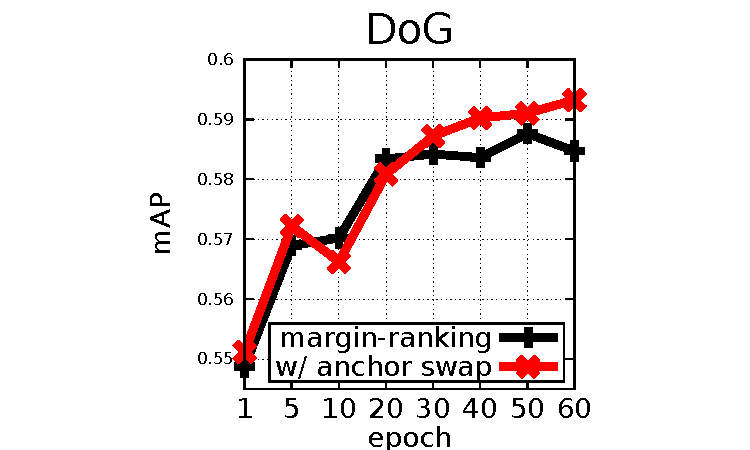
\includegraphics[trim={2.1cm 0 2.1cm 0},width=0.24\textwidth]{main/chapter02/images/dog_ranking}}
\subfigure{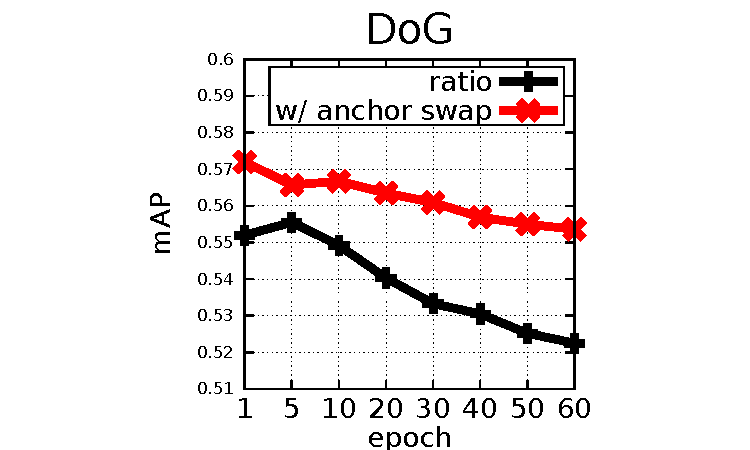
\includegraphics[trim={2.1cm 0 2.1cm 0},width=0.24\textwidth]{main/chapter02/images/dog_ratio}}
\subfigure{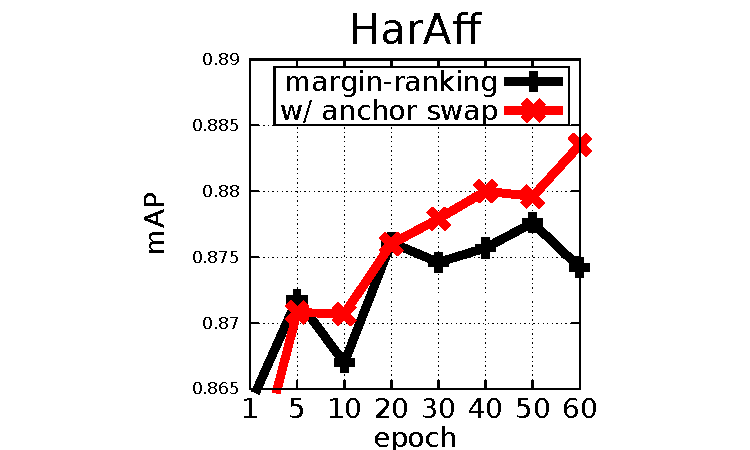
\includegraphics[trim={2.1cm 0 2.1cm 0},width=0.24\textwidth]{main/chapter02/images/haraff_ranking}}
\subfigure{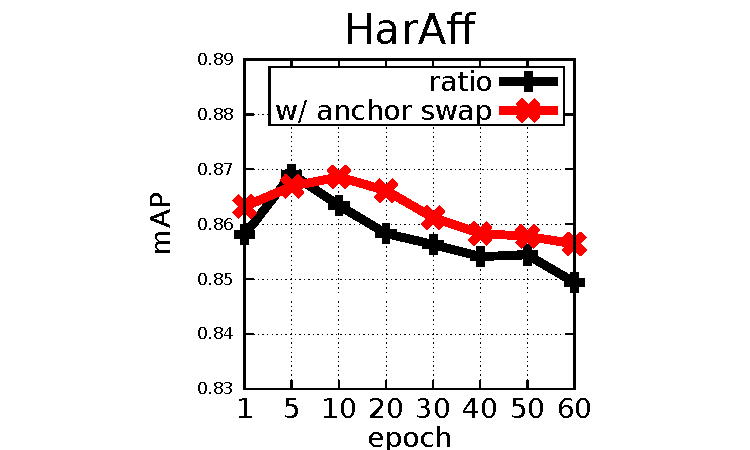
\includegraphics[trim={2.1cm 0 2.1cm 0},width=0.24\textwidth]{main/chapter02/images/haraff_ratio}}
\caption{Ratio based loss function overfits in the process of
   separating the positive and negative pairs within a
  triplet, and does not perform well in the nearest neighbour
  matching experiment. On the contrary, learning with triplets and
  margin ranking does not suffer from this problem which shows
  that ranking methods are more suitable for nearest neighbor
  matching scenarios.}
\label{fig:losses-vs}
\vspace{-0.1cm}
\end{figure}

\textbf{Keypoint matching}. Figure \ref{fig:oxford_results} presents the $mAP$ results for Oxford benchmark,
across all image sequences from the Oxford dataset, for two
different  keypoint detectors, DoG and Harris-Affine. Note that all
networks are trained on DoG keypoints. In the case of our ratio loss, we use the networks from the first epoch, since all the next
epochs would exhibit lower performance (cf. Fig~\ref{fig:losses-vs}).
In the case of the DoG keypoints, our networks outperform
all the others in terms of $mAP$. The second best performing
descriptor is the DeepDesc descriptor from \cite{simo2015deepdesc}. We
stress again here, that this descriptor was below the state of
the art in terms of ROC curves and FPR95 as shown in Table
\ref{tab:benchmark_brown}. This confirms our findings that the
classification benchmark is not a representative measure for the  common
real-world application of descriptors which often relies on nearest neighbor matching. When using
Harris-Affine keypoints our descriptor still outperforms the others,
although with a smaller margin.


\begin{figure}
\centering    
\subfigure{{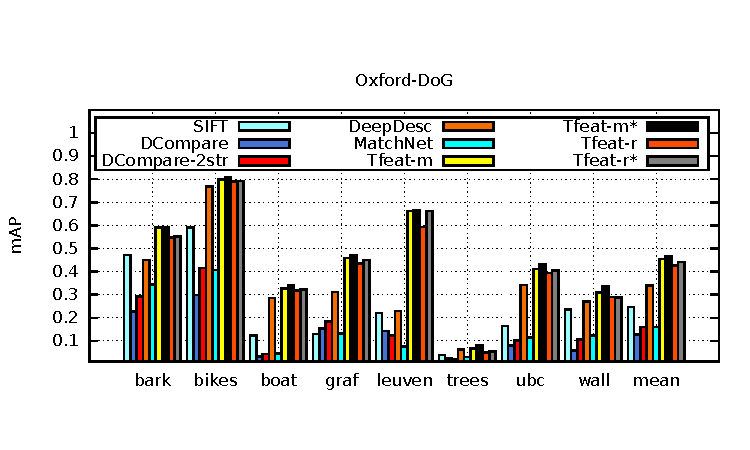
\includegraphics[trim={0.5cm 1.2cm 0.5cm 1.8cm},width=0.48\textwidth]{main/chapter02/images/oxford_dog}}}
\subfigure{{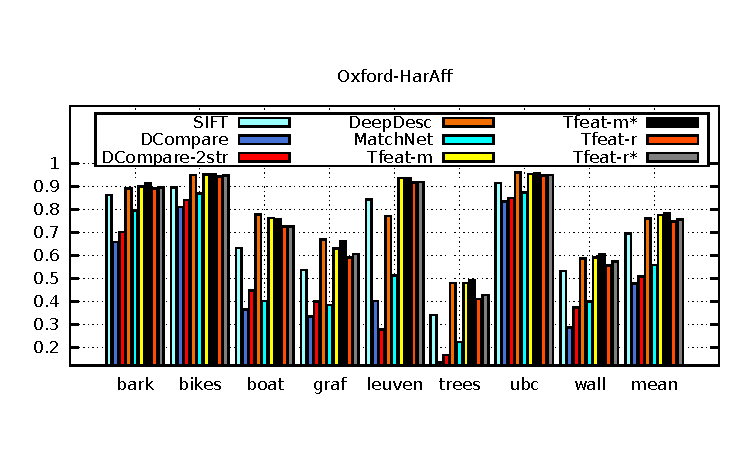
\includegraphics[trim={0.5cm 1.2cm 0.5cm 1.8cm},width=0.48\textwidth]{main/chapter02/images/oxford_haraff}}}
\caption{Evaluation on the Oxford image matching dataset
  \cite{schmid2003performance}, for two different types of feature
  extractors, DoG and  HarrisAffine.}
\label{fig:oxford_results}
\vspace{-0.2cm}
\end{figure}

\textbf{Image transformations.} Figure~\ref{fig:fischer_results} shows the results across various synthetic transformations of image pairs. Our descriptor gives the  top scores in most sequences. It is also worth noting, that even though this dataset has some severe deformations as well as nonlinear filtering, the overall performance for both types of feature extractors is higher than for the Oxford dataset. This shows that synthetic deformations are less challenging for descriptors than some real-world changes as the ones found in Oxford dataset.

\begin{figure}
\centering    
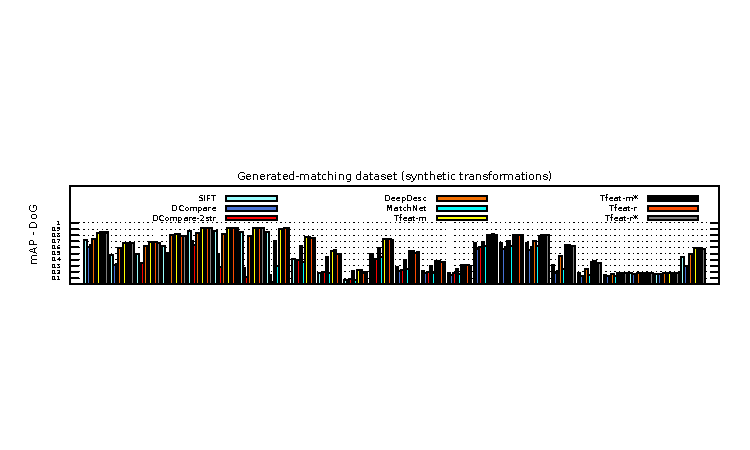
\includegraphics[trim={0.22cm 2.6cm 0.22cm 2.6cm},width=\textwidth]{main/chapter02/images/fischer_dog}
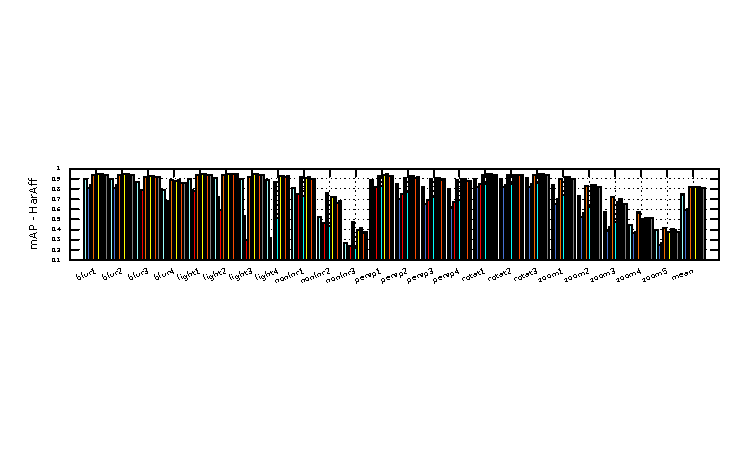
\includegraphics[trim={0.22cm 3cm 0.22cm 3cm},width=\textwidth]{main/chapter02/images/fischer_haraff}
\caption{Evaluation on the generated-matching dataset
  \cite{FDB14}, for two different types of feature
  extractors, DoG and  HarrisAffine.}
\label{fig:fischer_results}
\vspace{-0.2cm}
\end{figure}


\subsubsection{Efficiency}
One of the main motivations behind this work, was the need for a fast
and practical feature descriptor based on CNN. The small network trained with triplets
that we used in our experiments, is very
efficient in terms of descriptor extraction time.  We compare the extraction time
 per patch, averaged over $20K$ patches, of  recently
introduced convolutional feature descriptors. The extraction is done with NVIDIA Titan X GPU.
Our descriptor is 10 times faster than
DeepCompare \cite{ZagoruykoCVPR2015}, and 50 times faster than
MatchNet \cite{Han_2015_CVPR} and DeepDesc \cite{simo2015deepdesc}. In fact,
when running on GPU, we reach speeds of ${10\mu s}$ per patch which
is comparable with the CPU speeds of the fast binary
descriptors\cite{Calonder:2010:BBR:1888089.1888148}.  This is a
significant advantage over the previously proposed descriptors and
makes CNN based descriptors applicable to practical problems with
large datasets.

\subsection{Conclusion}
This work introduced a new approach to training CNN architecture for
extracting local image descriptors in the context of patch matching.
The results show that using triplets for training results in a better
descriptor and faster learning. The networks can be simplified and
extract features with a speed comparable to BRIEF.  Also the
dimensionality can be significantly reduced compared to other CNN
based descriptors. We show that due to these properties the proposed
network is less prone to over-fitting and has good generalisation
properties.  In addition, the high computational cost of hard negative
mining has been successfully replaced by the very efficient triplet
based loss.

We also demonstrate that ratio-loss based methods are more suitable
for patch pair classification, and margin-loss based methods work
better in nearest neighbour matching applications.  This indicates
that a good performance on patch classification does not necessarily
generalise to a good performance in nearest neighbour based
frameworks.

We provide all the learned models and the training code for all the
variants at \url{https://github.com/vbalnt/tfeat}. 
